%% LyX 2.2.1 created this file.  For more info, see http://www.lyx.org/.
%% Do not edit unless you really know what you are doing.
\documentclass[12pt,english]{article}
\usepackage[T1]{fontenc}
\usepackage[latin9]{luainputenc}
\usepackage[a4paper]{geometry}
\geometry{verbose,tmargin=1cm,bmargin=1cm,lmargin=1cm,rmargin=1cm}
\usepackage{graphicx}

\makeatletter

%%%%%%%%%%%%%%%%%%%%%%%%%%%%%% LyX specific LaTeX commands.
%% Because html converters don't know tabularnewline
\providecommand{\tabularnewline}{\\}
%% A simple dot to overcome graphicx limitations
\newcommand{\lyxdot}{.}


\makeatother

\usepackage{babel}
\begin{document}

\title{Introduction to Machine learning ( CS5011 )\\
Programming assignment \#3}

\author{Aravind S\\
EE14B013}

\date{14th Nov. 2016}
\maketitle

\section{Conversion}

ARFF is a popular format for data storage which is compatible with
many popular packages like Weka. It has 2 components, header and data.
\begin{itemize}
\item The header mentions the optional name and the data type of that feature.
Here, the first two attributes in all datasets are numerical and the
last attribute was categorical.
\item The dataset is a 2-dimensional dataset with labels associated with
every point.
\end{itemize}
As usual, I standardized the data before usage, which resulted in
better performance. This is to ensure that L2-norm is a proper distance
measure. It assumes the same weight given to both the features. As
a result, one feature should not dominate the other. Hence, standardizing
makes sure L2-norm is a good distance measure.

\section{Visualisation}

The standardized datasets have been visualised below.

\begin{figure}
\begin{minipage}[c][1\totalheight][t]{0.45\textwidth}%
\begin{center}
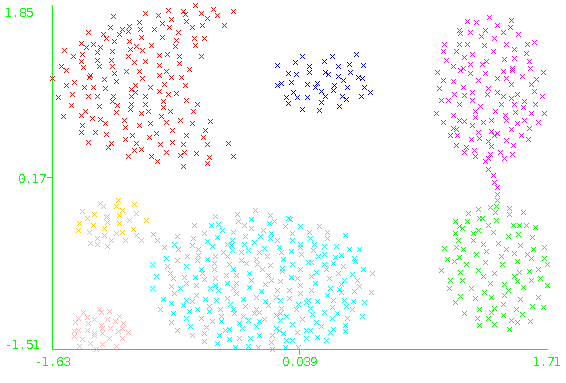
\includegraphics[scale=0.4]{/home/aravind/Desktop/myproj/ml-assgts/PA3/plots/Aggregation}
\par\end{center}
\caption{Aggregation}
%
\end{minipage}\hfill{}%
\begin{minipage}[c][1\totalheight][t]{0.45\textwidth}%
\begin{center}
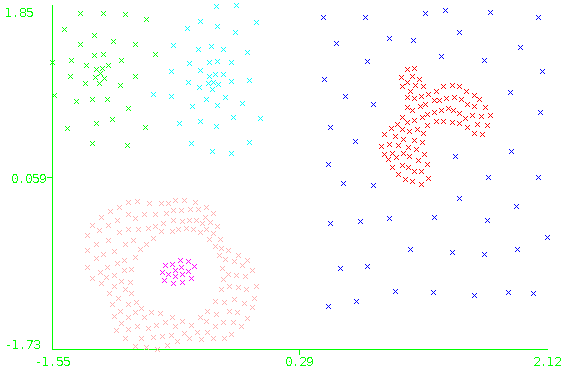
\includegraphics[scale=0.4]{/home/aravind/Desktop/myproj/ml-assgts/PA3/plots/Compound}
\par\end{center}
\caption{Compound}
%
\end{minipage}
\end{figure}

\begin{figure}
\begin{minipage}[c][1\totalheight][t]{0.45\textwidth}%
\begin{center}
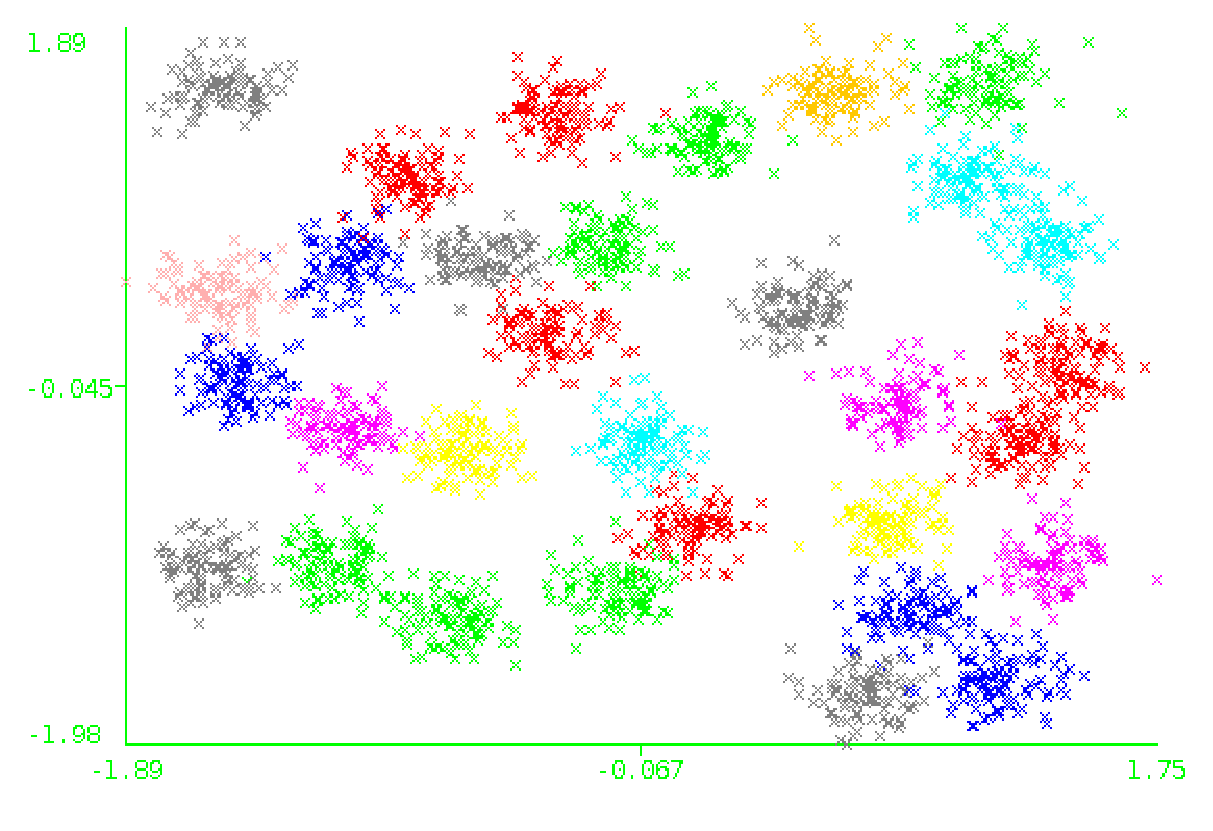
\includegraphics[scale=0.4]{/home/aravind/Desktop/myproj/ml-assgts/PA3/plots/D31}
\par\end{center}
\caption{D31}
%
\end{minipage}\hfill{}%
\begin{minipage}[c][1\totalheight][t]{0.45\textwidth}%
\begin{center}
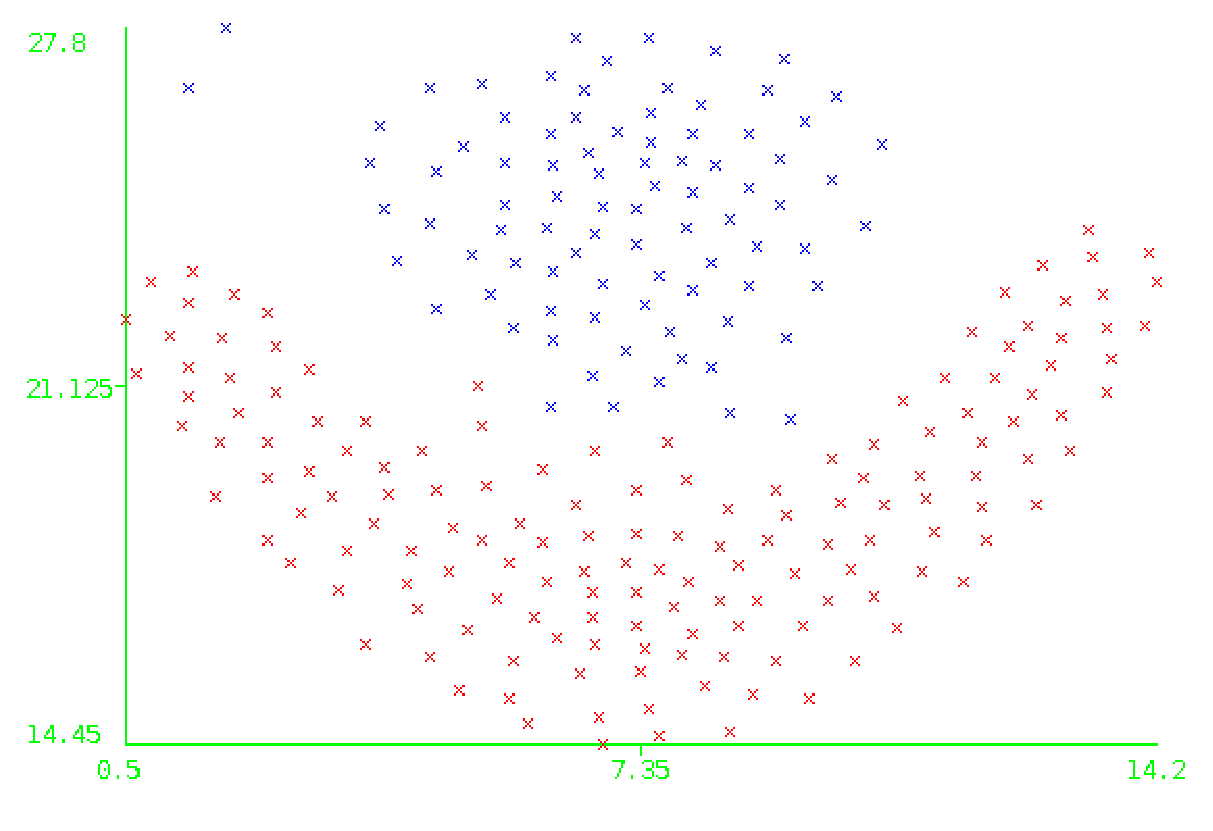
\includegraphics[scale=0.4]{/home/aravind/Desktop/myproj/ml-assgts/PA3/plots/flame}
\par\end{center}
\caption{Flames}
%
\end{minipage}
\end{figure}

\begin{figure}
\begin{minipage}[c][1\totalheight][t]{0.45\textwidth}%
\begin{center}
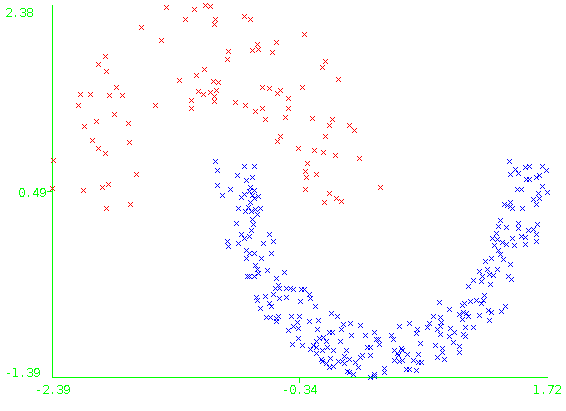
\includegraphics[scale=0.4]{/home/aravind/Desktop/myproj/ml-assgts/PA3/plots/jain}
\par\end{center}
\caption{Jain}
%
\end{minipage}\hfill{}%
\begin{minipage}[c][1\totalheight][t]{0.45\textwidth}%
\begin{center}
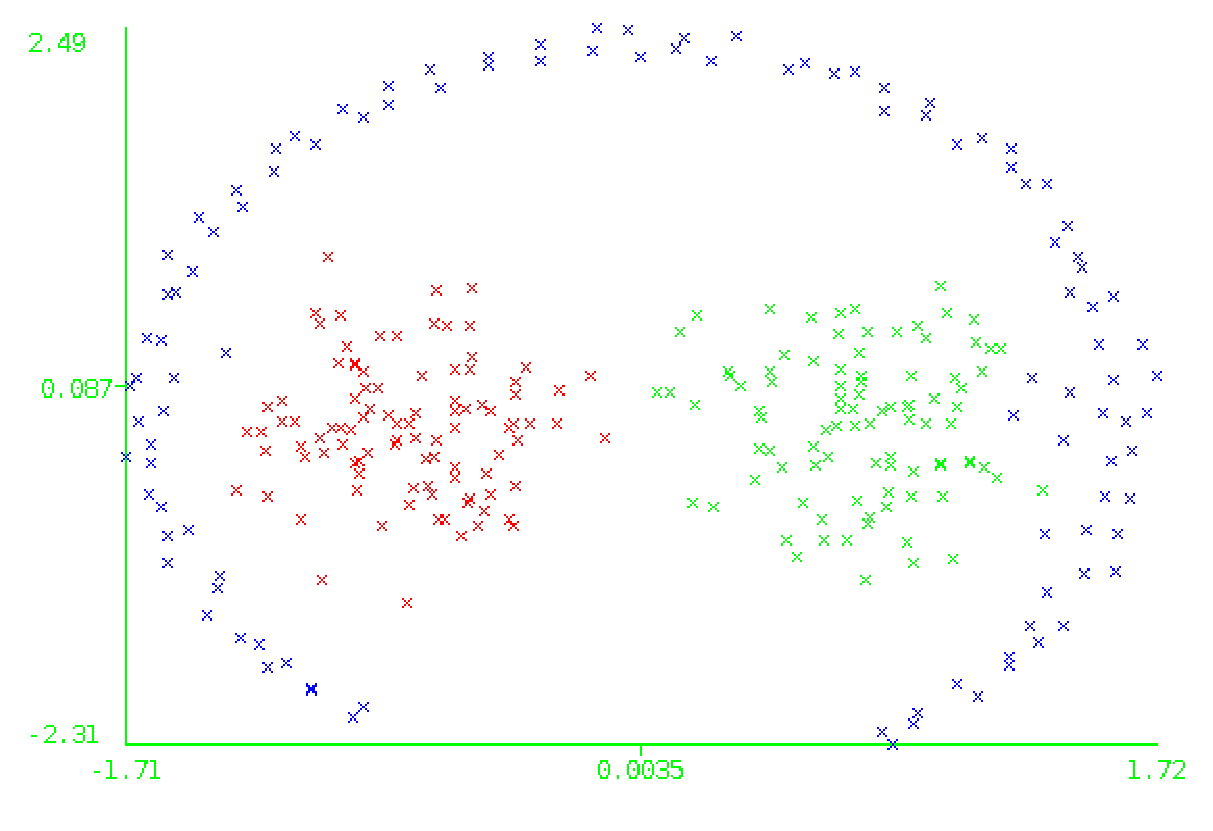
\includegraphics[scale=0.4]{/home/aravind/Desktop/myproj/ml-assgts/PA3/plots/pathbased}
\par\end{center}
\caption{Path-based}
%
\end{minipage}
\end{figure}

\begin{figure}
\begin{minipage}[c][1\totalheight][t]{0.45\textwidth}%
\begin{center}
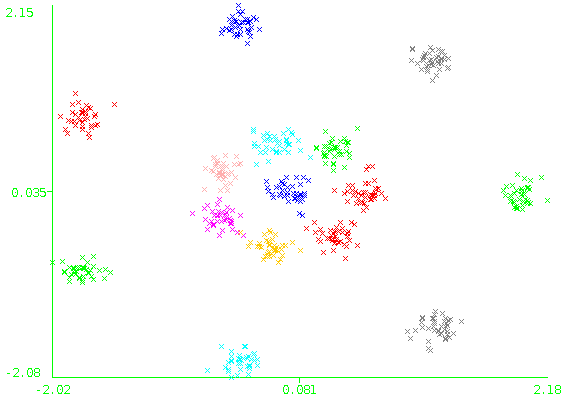
\includegraphics[scale=0.4]{/home/aravind/Desktop/myproj/ml-assgts/PA3/plots/R15}
\par\end{center}
\caption{R15}
%
\end{minipage}\hfill{}%
\begin{minipage}[c][1\totalheight][t]{0.45\textwidth}%
\begin{center}
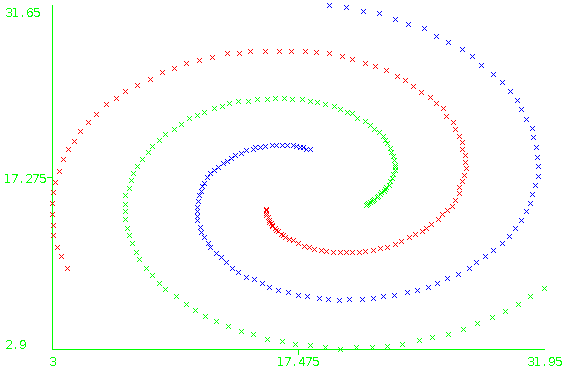
\includegraphics[scale=0.4]{/home/aravind/Desktop/myproj/ml-assgts/PA3/plots/spiral}
\par\end{center}
\caption{Spiral}
%
\end{minipage}
\end{figure}


\subsection*{Which algorithm to choose?}
\begin{itemize}
\item K-means clustering works well for datasets with convex clusters.
\item Hierarchical clustering ( HC ) with complete link meta-distance forces
the obtained clusters to be spherical in nature. As a result, this
works well for datasets with convex clusters.
\item DBSCAN obtains non-convex clusters, but it requires good separation
between two clusters ( otherwise the optimal (min pts, $\epsilon$)
is difficult to obtain ).
\item Hierarchical clustering with single link meta-distance also obtains
non-convex clusters. It is better than DBSCAN as we can specify the
number of clusters needed, and hence more robust to noise in the datasets.
\end{itemize}
Having known this, we can obtain a qualitative estimate about which
clustering algorithm performs well on the given dataset.

\subsubsection*{Aggregation}

Since the points are nearly convex, K-means and HC-complete will work
well. HC-single will work well except for the region between the clusters,
which may get misclassified. DBSCAN works provided we have a high
value for minpoints. This prevents the boundary points getting classified
as outliers.

\subsubsection*{Compound}

K-means and HC-complete will not work due to non-convex nature of
certain clusters. DBSCAN will work for certain value of min-pts but
might merge the points on the right ( the non-convex cluster points
and the less-densely placed points surrounding it ). HC-single will
also work as it obtains non-convex clusters, but might merge the above
mentioned clusters.

\subsubsection*{D31}

Since, the clusters are convex, K-means and HC-complete will work
well. But results might be slightly different due to noisy points
near the cluster boundary. DBSCAN will not work as the clusters are
not well separated and there are a lot of noisy/overlapping points.
Similarly, HC-single will suffer. But its output might be slightly
better as we can specify the number of clusters we want, which can
give a better partition between clusters.

\subsubsection*{Flames}

K-means and HC-complete will not work due to non-convex clusters.
Since the clusters are almost of uniform density and are well separated,
DBSCAN and HC-single will work. It is necessary to choose the appropriate
minpoints for DBSCAN.

\subsubsection*{Jain}

K-means and HC-complete will not work well, as the clusters are not
convex. Since, the clusters are well separated, DBSCAN and HC-single
will work well. The performance here will be better than Flames as
the clusters are better separated.

\subsubsection*{Path-based}

Due to non-convex nature of clusters, K-means and HC-complete will
not perform well. On the other hand, HC-single and DBSCAN will perform
well on this dataset. Choosing wrong values of $\epsilon$ for DBSCAN
might result in misclassification near boundary points. On the other
hand, HC-single will perform better as there are no parameters to
tune in it, except the number of clusters.

\subsubsection*{R15}

The dataset has convex clusters and are well separated ( unlike D31
). So, all algorithms will work well.

\subsubsection*{Spiral}

Owing to the non-convex nature of clusters, DBSCAN and HC-single will
work well for this dataset. K-means and HC-complete will not perform
well on this dataset.

\section{Performance of K-means on R15 dataset}

For $k=8$, the cluster purity is $0.533$. The assigned clusters
is shown below.\\
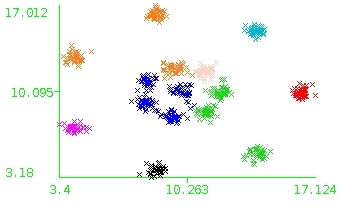
\includegraphics{/home/aravind/Desktop/myproj/ml-assgts/PA3/task-c/R15-Kmeans-8}\\
\\
As the cluster size increases, the purity increases as well. This
is because, the clusters are becoming more and more skewed. Theoritically,
the cluster purity is $1.0$ if $k=n$, where $k$ is the number of
clusters and $n$ is the number of data points.\\
\\

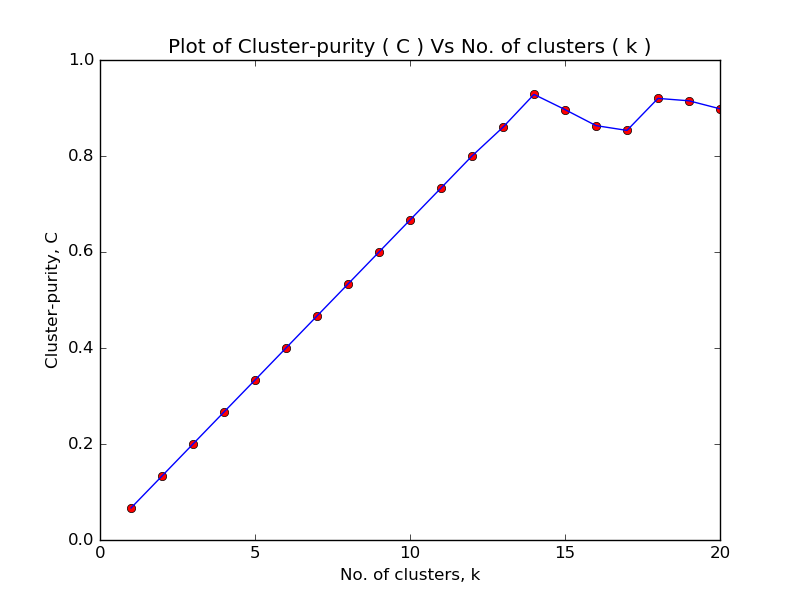
\includegraphics[scale=0.7]{/home/aravind/Desktop/myproj/ml-assgts/PA3/task-c/plot-cluster-purity-vs-k}

\section{Performance of DBSCAN on the Jain dataset}

As we all know, DBSCAN is very sensitive to parameters $(minpoints,\epsilon)$.
Wrong choices of the parameters gives horrible clustering results.
In order to obtain the correct choice of the parameters, I resolved
to a grid-search over the $(minpoints,\epsilon)$ space. I observed
that the variation of cluster-purity with the parameters is not predictable.
So, I am reporting all the results observed.\\
\\
I varied $\epsilon$ from $0$ to $1$ in steps of $0.05$ and $minpoints$
from $1$ to $20$ in steps of $1$. Once an optimal range for $\epsilon$
and $minpoints$ are obtained, the values are finetuned to get best
performance. The following observations were made.
\begin{itemize}
\item For large values of $\epsilon$, DBSCAN identifies a large number
of core points and as a result classifies the entire data into a single
cluster. This resulted in a cluster purity of around $0.74$. The
visualisation shown below was obtained for $minpoints=11$ and $\epsilon=0.9$.
Note, no points were flagged as OUTLIERS.\\
\\
\includegraphics{/home/aravind/Desktop/myproj/ml-assgts/PA3/task-d/jain-0\lyxdot 9-11-0\lyxdot 74}
\item For large values of $minpoints,$ less number of core points are identified
and hence, many points are flagged as NOISE.
\item Excluding the above configurations, the reasonable range of values
are $minpoints$ between $11$ and $17$ and $\epsilon$ around $0.1$.
\item The best purity for $2$ clusters was obtained, when $\epsilon=0.08$
and $minpoints=2$, for which the purity was $0.9785$. This resulted
in $8$ outliers and the remaining clustered. The results are visualised
below.\\
\\
\includegraphics{/home/aravind/Desktop/myproj/ml-assgts/PA3/task-d/jain-0\lyxdot 08-2-0\lyxdot 9785}
\end{itemize}

\section{DBSCAN Vs Hierarchical clustering on Path-based, Spiral and Flames
datasets}

\subsection*{DBSCAN}

To obtain the optimal values of $\epsilon$ and $minpoints$, grid-search
is followed. I varied $\epsilon$ from $0$ to $1$ in steps of $0.05$
and $minpoints$ from $1$ to $20$ in steps of $1$. Once an optimal
range for $\epsilon$ and $minpoints$ are obtained, the values are
finetuned to get best performance. The following observations were
made. The rough range for $\epsilon$ was around $0.1$ and for $minpoints$,
it is $2$ to $9$. The results are tabulated below.

\begin{tabular}{|c|c|c|c|c|c|c|}
\hline 
\multicolumn{7}{|c|}{Performance of DBSCAN on the Path-based, Spiral and Flames datasets}\tabularnewline
\hline 
\hline 
\textbf{Dataset} & \textbf{Classes} & \textbf{Epsilon $\epsilon$} & \textbf{Minpoints $M$} & \textbf{Clusters} & \textbf{Outliers} & \textbf{Purity}\tabularnewline
\hline 
Path-based & 3 & 0.07 & 9 & 3 & 107 & 0.9933\tabularnewline
\hline 
Spiral & 3 & 0.1 & 2 & 3 & 0 & 1.0\tabularnewline
\hline 
Flames & 2 & 0.1 & 9 & 2 & 3 & 0.9875\tabularnewline
\hline 
\end{tabular}

\subsection*{Hierarchical clustering}

Weka supports a number of linkTypes like \textbf{single, complete,
average, mean, centroid, ward, adjcomplete and neighbour\_joining.
}Generally for non-convex clusters, \textbf{ward }and \textbf{single}
link types prove to be efficient in clustering.\\
\\
After experimenting with all possible link types, the results are
summarised below.\\

\begin{tabular}{|c|c|c|c|}
\hline 
\multicolumn{4}{|c|}{Performance of Hierarchical clustering on the Path-based, Spiral and
Flames datasets}\tabularnewline
\hline 
\hline 
\textbf{Dataset} & \textbf{Clusters} & \textbf{Link type} & \textbf{Purity}\tabularnewline
\hline 
Path-based & 3 & Ward & 0.7534\tabularnewline
\hline 
Spiral & 3 & Single & 1.0\tabularnewline
\hline 
Flames & 2 & Ward & 1.0\tabularnewline
\hline 
\end{tabular}\\
\\
The above results are visualised below.

\begin{figure}
\begin{minipage}[c][1\totalheight][t]{0.45\textwidth}%
\begin{center}
\includegraphics[scale=0.4]{/home/aravind/Desktop/myproj/ml-assgts/PA3/task-e/pathbased-dbs-0\lyxdot 07-9-0\lyxdot 9933}
\par\end{center}
\caption{Path-based ( DBSCAN )}
%
\end{minipage}\hfill{}%
\begin{minipage}[c][1\totalheight][t]{0.45\textwidth}%
\begin{center}
\includegraphics[scale=0.4]{/home/aravind/Desktop/myproj/ml-assgts/PA3/task-e/pathbased-hc-ward-0\lyxdot 7534}
\par\end{center}
\caption{Path-based ( Hierarchical clustering )}
%
\end{minipage}
\end{figure}

\begin{figure}
\begin{minipage}[c][1\totalheight][t]{0.45\textwidth}%
\begin{center}
\includegraphics[scale=0.4]{/home/aravind/Desktop/myproj/ml-assgts/PA3/task-e/spiral-dbs-0\lyxdot 1-2-1\lyxdot 0}
\par\end{center}
\caption{Spiral ( DBSCAN )}
%
\end{minipage}\hfill{}%
\begin{minipage}[c][1\totalheight][t]{0.45\textwidth}%
\begin{center}
\includegraphics[scale=0.4]{/home/aravind/Desktop/myproj/ml-assgts/PA3/task-e/spiral-hc-single-1\lyxdot 0}
\par\end{center}
\caption{Spiral ( Hierarchical clustering )}
%
\end{minipage}
\end{figure}

\begin{figure}
\begin{minipage}[c][1\totalheight][t]{0.45\textwidth}%
\begin{center}
\includegraphics[scale=0.4]{/home/aravind/Desktop/myproj/ml-assgts/PA3/task-e/flames-dbs-0\lyxdot 1-9-0\lyxdot 9875}
\par\end{center}
\caption{Flames ( DBSCAN )}
%
\end{minipage}\hfill{}%
\begin{minipage}[c][1\totalheight][t]{0.45\textwidth}%
\begin{center}
\includegraphics[scale=0.4]{/home/aravind/Desktop/myproj/ml-assgts/PA3/task-e/flames-hc-ward-1\lyxdot 0}
\par\end{center}
\caption{Flames ( Hierarchical clustering )}
%
\end{minipage}
\end{figure}


\section{Analysis of D31 dataset}

\subsection*{K-means}

The performance of K-means is tabulated below. We can observe that
K-means successfully identifies the $32$ clusters for $k=32$ with
a cluster-purity of $0.879$. The purity increases as we increase
$k$. But, it saturates for large $k$. For instance, beyond $k=64$,
the value of cluster-purity remains almost constant around $0.966$.\\
\\

\begin{tabular}{|c|c|}
\hline 
\multicolumn{2}{|c|}{Variation of cluster-purity with k}\tabularnewline
\hline 
\hline 
No. of clusters $k$ & Cluster purity\tabularnewline
\hline 
32 & 0.879\tabularnewline
\hline 
40 & 0.897\tabularnewline
\hline 
48 & 0.957\tabularnewline
\hline 
56 & 0.965\tabularnewline
\hline 
64 & 0.967\tabularnewline
\hline 
128 & 0.966\tabularnewline
\hline 
\end{tabular}

\subsection*{DBSCAN}

We can observe that the clusters are not well separated. As a result,
DBSCAN doesn't perform well. I did a grid-search by varying $\epsilon$
from $0$ to $1$ in steps of $0.05$ and varying $minpoints$ from
$1$ to $20$ in steps of $1$. As the clusters overlap, the number
of clusters obtained is less. In all my trials, it doesn't exceed
$5$.\\
\\
The best cluster purity obtained was $0.1622$ for $\epsilon=0.05$
and $minpoints=11$.

\subsection*{Hierarchical clustering}

Using the Ward's linkage with $32$ clusters we get a cluster-purity
of $0.9632$. It is visualised below.\\

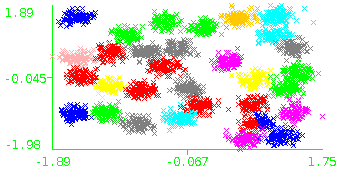
\includegraphics{/home/aravind/Desktop/myproj/ml-assgts/PA3/task-f/d31-hc-ward}
\end{document}
